\documentclass{standalone}
\usepackage{tikz}
\usetikzlibrary{calc} % for tikz calculations
\usetikzlibrary{arrows,decorations.markings} % make arrow head bigger

% set up externalization
\usetikzlibrary{external}
\tikzset{external/system call={latex \tikzexternalcheckshellescape -halt-on-error
-interaction=batchmode -jobname "\image" "\texsource" && 
dvips -o "\image".ps "\image".dvi &&
ps2eps "\image.ps"}}
\tikzexternalize[shell escape=-enable-write18] % MikTeX uses a -enable-write18 instead of --shell-escape.
% compile with: latex -enable-write18

\begin{document}

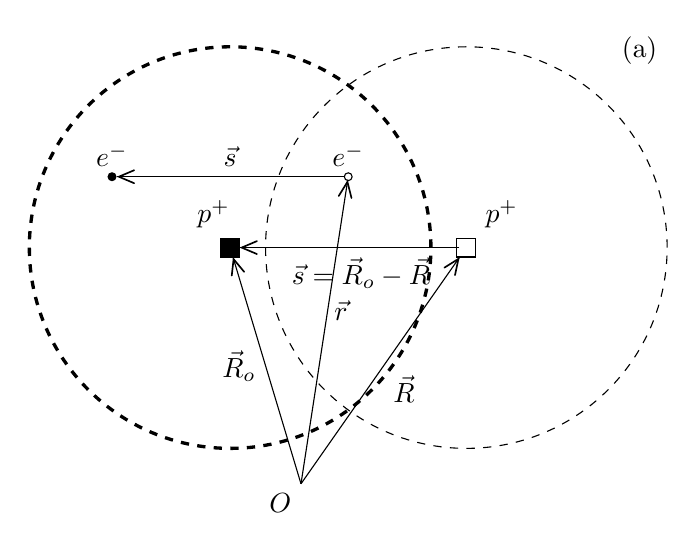
\begin{tikzpicture}
% define arrow head
[
    decoration={
      markings,
      mark=at position 1 with {\arrow[scale=1.5,black]{angle 45}};
    }
]

% scale
\pgfmathsetmacro{\a}{3}
\coordinate (H1) at (0,0);
\coordinate (H) at (\a,0);

% coordinate
\coordinate (O) at ($0.5*(H1)+0.3*(H)-(0,\a)$);
\node at (O) [below left]{$O$};

% ions
\pgfmathsetmacro{\R}{0.04*\a} % ion radius
\draw[fill] ($(H1)-(\R,\R)$) rectangle ($(H1)+(\R,\R)$) node [above left] {$p^+$};
\draw ($(H)-(\R,\R)$) rectangle ($(H)+(\R,\R)$) node [above right] {$p^+$};
\draw[postaction={decorate}] (O) -- ($0.96*(H)+0.04*(O)$);
\node at ($0.5*(H)+0.5*(O)$) [below right] {$\vec{R}$};
\draw[postaction={decorate}] (O) -- ($0.96*(H1)+0.04*(O)$);
\node at ($0.5*(H1)+0.5*(O)$) [left] {$\vec{R}_o$};

% wave function contour
\draw[very thick,dashed] (H1) circle (0.85*\a);
\draw[dashed] (H) circle (0.85*\a);

\coordinate (e) at (.5*\a,.3*\a);
\coordinate (e1) at ($(e)-(H)$);

% electrons
\node[draw,circle,inner sep=1pt] at (e) {};
\node at (e) [above] {$e^-$};
\node[draw,circle,inner sep=1pt,fill] at (e1) {};
\node at (e1) [above] {$e^-$};

% vectors
\draw[postaction={decorate}] (O) -- ($0.99*(e)+0.01*(O)$);
\node at ($0.5*(e)+0.5*(O)$) [above right] {$\vec{r}$};
\draw[postaction={decorate}] ($0.97*(H)$)--($0.04*(H)$);
\node at ($0.5*(H1)+0.22*(H)$) [below right] {$\vec{s}=\vec{R}_o-\vec{R}$};

\draw[postaction={decorate}] ($(e)-(0.02*\a,0)$) -- ($(e1)+(0.02*\a,0)$);
\node at ($0.5*(e)+0.5*(e1)$) [above] {$\vec{s}$};
%\draw[postaction={decorate}] (O) -- ($0.99*(e1)+0.01*(O)$);
%\node at ($0.5*(O)+0.5*(e1)$) [below left] {$\vec{r'}$};

% subplot marking
\node at (5.2,2.5) {(a)};

\end{tikzpicture}

\end{document}